\section{Finding The Best Approximation}
\label{sec:search}

Our problem may be solved na\"{\i}vely by an exhaustive search over the possible refinements. However, the search space of refinements becomes intractably large even with relatively modest datasets, as the number of possible refinements is exponential in the number of the query's attributes.
Beyond the high cost of an exhaustive search, a na\"{\i}ve solution would require the evaluation of each refinement query on the DBMS to check its deviation from the constraint set. 

To address these challenges, we propose a solution based on a mixed-integer linear program (MILP). Mixed-integer linear programming is a model for optimizing a linear objective function subject to a set of expressions (equalities and inequalities) linear in the discrete or continuous variables of the problem, limiting the space of feasible assignments. Solvers for such programs have been developed with techniques to solve even large problems efficiently in practice, as discussed in \cite{QFix}.
By incorporating the concepts introduced in~\cite{MLJ22, ERICA}, we utilize data annotations to depict potential refinements. These annotations serve as variables in the MILP, and enable us to quantify the deviation from the constraint set without having to reevaluate refinements across the DBMS.

Briefly, a solution for a MILP is an assignment for the variables in the expressions, such that they are satisfied and the objective function is minimized. 
Intuitively, given a database $D$, a query $Q$, a constraint set $\constraints$, a maximum deviation from the constraint set $\varepsilon \geq 0$, and a distance measure $DIS$, we construct an instance of MILP such that the solution corresponds to a minimal refinement that produces a ranking such that its deviation is within the maximum deviation $\varepsilon$ from the constraint set $\constraints$ while minimizing $DIS$.
By formulating \problem{} as a MILP, we can leverage existing tools to streamline the search process. 


It is important to note that by using MILP to represent the problem, we are limited to distance measures that can be modeled by a linear program. However, this limitation still allows a wide range of useful distance measures, including the ones defined in~\Cref{sec:distance}. Some of these measures may require additional modeling techniques to become linearized. For example, when modeling the Jaccard distance, we can use the Charnes-Cooper transformation~\cite{CC62}. Similarly, we can introduce auxiliary  variables to model the version of Kendall's $\tau$ for top-$k$ lists introduced in \cite{FKS03}. %

\begin{table}[t!]
    \centering
    \caption{Summary of variables used in our MILP model}
    \footnotesize
    \begin{tabularx}{0.7\textwidth}{ccX}
    \hline
    {\bf Var.} & {\bf Domain} & {\bf Description} \\
    \hline
    $C_{A,\diamond}$  & $\mathbb{R}$ & Refined $C$ for a num. predicate on $A$ with operator $\diamond$                     \\
    $A_v$             & $\{0, 1\}$ & Whether a value $v$ is selected by the cat. predicate on $A$                           \\
    $A_{v, \diamond}$ & $\{0, 1\}$ &  Whether a value $v$ is in the range of the num. predicate on $A$ with operator $\diamond$ \\
    $r_t$            & $\{0, 1\}$ & Whether tuple $t$ is selected by the refinement                                     \\
    $s_{t}$          & $\mathbb{R}$ & Rank of tuple $t$ in the ranking generated by the refinement                              \\
    $l_{t, k}$       & $\{0, 1\}$ & Whether tuple $t$ is present in the top-$k$ of the ranking generated by the refinement          \\
    $E_{G, k}$       & $\mathbb{R}$ & Number of tuples to add (remove) to satisfy lower-bound (upper-bound) cardinality constraint    \\
    \hline
    \end{tabularx}
    \label{tab:variables}
\end{table}

The MILP instance we construct consists of two main groups of expressions: those that require that all tuples selected by the refinement are in the ranking according to the {\tt ORDER BY} expression of $Q$, and those that enforce that the derived ranking's deviation from the constraint set does not exceed the input bound $\varepsilon$. We next explain the construction of the expressions in each set, and, in order to give a more intuitive picture of the process, demonstrate in \Cref{fig:example_summary} how variables are generated from a running example and how they are combined by these expressions.


\subsection{Modeling Refinement Output Using Expressions}

Inspired by the use of provenance for query refinements~\cite{MLJ22,ERICA}, we utilize the notion of data annotations to model refinements through a set of expressions. This set is divided into two parts. The first part is used to model the tuples that satisfy the refinement query's predicates, while the second part ensures that the selected tuples are ordered correctly by the {\tt ORDER BY} expression of the input query. We start by describing the variables used in the expressions.



		

\begin{table}%
        \centering	
  \caption{$\widetilde{Q}$ obtained from \running{}}
  \hspace*{-1cm}
        \footnotesize
		\begin{tabular}{clccc}
		\cline{2-5}
		& \textbf{ID} & \textbf{Gender} & \textbf{Income} &  $\prov(t)$ \\ \cline{2-5}
		 & $t_1$           & M               & Medium         & $\{Activity_{SO}, GPA_{3.7}\}$\\    
		 & $t_2$           & F               & Low         & $\{Activity_{SO}, GPA_{3.8}\}$\\    
		 & $t_3$           & F               & Low        & $\{Activity_{GD}, GPA_{3.6}\}$\\    
		& $t_4$            & M               & High     & $\{Activity_{RB}, GPA_{3.8}\}$\\
         & $t_4'$           & M               & High & $\{Activity_{TU}, GPA_{3.8}\}$\\
		 & $t_5$           & F               & Medium   & $\{Activity_{MO}, GPA_{3.6}\}$\\    
		& $t_6$            & F               & Low       & $\{Activity_{SO}, GPA_{3.7}\}$ \\    
		 & $t_7$           & M               & Low       & $\{Activity_{RB}, GPA_{3.7}\}$ \\    
		 & $t_8$           & F               & High      & $\{Activity_{RB}, GPA_{3.9}\}$\\
         & $t_{8}'$           & F               & High       & $\{Activity_{TU}, GPA_{3.9}\}$\\
		 & $t_{10}$           & M               & High  & $\{Activity_{RB}, GPA_{3.7}\}$\\    
		 & $t_{11}$           & F               & Low    & $\{Activity_{RB}, GPA_{3.8}\}$\\    
		 & $t_{12}$           & M               & Medium    & $\{Activity_{RB}, GPA_{4.0}\}$\\    
  	 &  $t_{14}$            & F               & Low       & $\{Activity_{RB}, GPA_{3.7}\}$\\ \cline{2-5} 
		\end{tabular}
  \label{tab:joined}
\end{table}

\paragraph*{\textbf{Variables}} Given a query $Q$ and a database $D$, for each categorical predicate in $\cat(Q)$ over an attribute $A$, we define a variable $A_{v} \in \{0, 1\}$ for each value $v$ in the domain of $A$ in $D$. Intuitively, a solution to the MILP where $A_{v} = 1$ corresponds to a refinement that includes $A = v$ in the categorical predicates. For each numerical predicate $A \diamond C \in \num(Q)$, we define a variable $C_{A, \diamond}$ whose value is in the range of values of $A$ in $D$, and a set of variables $A_{v, \diamond}$ for each value $v$ in the domain of $A$ in $D$.

\begin{example}
$Activity_{RB}$ and $Activity_{SO}$ are two of the variables generated by the categorical predicate {\tt Activity = `RB'}
since these values are present in the database. 
The variable $C_{GPA, \geq}$ is generated from the numerical predicate {\tt GPA >= 3.7}. Additionally, the variable $GPA_{3.7, \geq}$ is generated since there exists a tuple in the data with the value $3.7$ in the {\tt GPA} attribute. 
\end{example} 

The value of $C_{A, \diamond}$ represents the value of the constant $C$ in the refinement query, and the variables $A_{v, \diamond}$ are used to determine whether a given tuple $t$ in $D$ (with the value $v$ in $A$) satisfies that predicate over $A$ in the refined query. More concretely, the variable $A_{v, \diamond}$ is used to reflect whether  $v \diamond C_{A, \diamond}$. Finally, we use a variable $r_t$ to denote the existence of a tuple $t$ in the output of a refinement query and a variable $s_t$ to indicate the position of $t$ in the output.



\paragraph*{\textbf{Expressions}}  We formulate a set of expressions such that the assignment generated by a solver to the MILP instance corresponds to the set of tuples selected by the corresponding refinement query. A tuple is part of a query's output if it satisfies its predicates set. We first define expressions for numerical predicates. Intuitively, a tuple $t$ with value $v$ in attribute $A$ satisfies the predicate $A \diamond C_{A, \diamond}$ if $v \diamond C_{A, \diamond}$. For lower-bound predicates, i.e., when $A \geq C$ or $A > C$, we model this using the following MILP expressions for each predicate in $\num(Q)$ and each value $V$ in the domain of $A$ in~$D$.%
\begin{align}
\begin{split}
C_{A, \diamond} + M_A \cdot A_{v, \diamond} &\geq v + (1 - {\sf St}(\diamond)) \cdot \delta \label{eq:value_bounds_inline}\\
C_{A, \diamond} - M_A \cdot (1 - A_{v, \diamond}) &\leq v - {\sf St}(\diamond) \cdot \delta
\end{split}
\end{align} 
where $M_A$ is a constant larger than the maximum absolute value in the domain of the attribute $A$ in $D$, ${\sf St}(\diamond)$ is $1$ if $\diamond$ is a strict inequality and $0$ otherwise, and $\delta$ is some small constant added when $\diamond$ is strict in order to relax the inequality as MILP expressions do not support strict inequalities. We choose $\delta$ to be smaller than the smallest pairwise difference between the values in the domain of $A$, ensuring the relaxation does not include another value from the domain. For upper-bound predicates, we instead use the following set of expressions.
\begin{align}
\begin{split}
C_{A, \diamond} - M_A \cdot A_{v, \diamond} &\leq v - (1 - {\sf St}(\diamond)) \cdot \delta \label{eq:value_bounds_inline2}\\
C_{A, \diamond} + M_A \cdot (1 - A_{v, \diamond}) &\geq v + {\sf St}(\diamond) \cdot \delta
\end{split}
\end{align}
 Intuitively, the first expressions in (\ref{eq:value_bounds_inline}) and (\ref{eq:value_bounds_inline2}) ensure that $A_{v, \diamond}$ is $1$ if $v \diamond C_{A, \diamond}$ is true and the second expressions are used to ensure that $A_{v, \diamond}$ is 0 if $v \diamond C_{A, \diamond}$ is false. Together, they enforce that $A_{v, \diamond}$ is $1$ if and only if $v \diamond C_{A, \diamond}$ is true.


\begin{example}
\label{ex:numeric_constraint}
Continuing with our example, the following expressions are generated using the variables $C_{GPA, \geq}$ and $GPA_{3.7, \geq}$ for the numerical predicate {\tt GPA $\geq$ 3.7} in the \running{}.
\begin{align*}
    C_{GPA, \geq} + 5 \cdot GPA_{3.7, \geq} \geq 3.701 \\ 
    C_{GPA, \geq} - 5 \cdot (1 - GPA_{3.7, \geq}) \leq 3.7
\end{align*}
Here $M_A$ is set to $5$, a value greater than any value of the attribute {\tt GPA} in the data, and ${\sf St}(\diamond)$ is $0$ (since the inequality in the predicate is not strict). Consider an assignment that assigns the $3.7$ to $C_{GPA, \geq}$. This assignment corresponds to a query with the predicate {\tt GPA $\geq$ 3.7}. Assigning this value to the above expression results in 
\begin{align*}
    3.7 + 5 \cdot GPA_{3.7, \geq} \geq 3.701 \\ 
    3.7 - 5 \cdot (1 - GPA_{3.7, \geq}) \leq 3.7
\end{align*}
In this case, the value of $GPA_{3.7, \geq}$ should be $1$ as well, indicating that tuples with a value $\geq 3.7$ in the {\tt GPA} attribute meet the condition. Indeed, these expressions can be satisfied if and only if the variable $GPA_{3.7, \geq}$ is assigned the value $1$. Notice that adding $\delta$ in the first expression is necessary in order to guarantee that the only valid assignment for $GPA_{3.7, \geq}$ is $1$. 



\end{example}













Next, we construct expressions that model the existence of a tuple in the query's output (represented using the variable $r_t$). The expressions should be able to model any possible refinement. Note that the output of a refinement may include tuples that are not part of the output of the original query. To this end, we use $\widetilde{Q}$ to denote the query obtained from $Q$ by omitting the selection predicates and any {\tt DISTINCT} statement. Intuitively, the output of $\widetilde{Q}$ over $D$ contains the output of every possible refinement query. A tuple $t$ is in the output of a query $Q$ if $t$ satisfies all the predicates in $Q$. 
To indicate whether $t$ is part of the output, we leverage the notion of {\it lineage}. The lineage of a tuple $t\in\widetilde{Q}(D)$ is the set of variables $A_v$ and $A_{v, \diamond}$ that correspond to the values of $t$ for each attribute in $\attr(Q)$: $\prov(t)=\{A_{t.A} \mid \forall \left( \bigvee_{c \in C} A = c \right) \in \cat(Q)\}~ \cup~ \{A_{t.A, \diamond} \mid \forall (A \diamond C) \in \num(Q)\}$. Table~\ref{tab:joined} shows the result of $\widetilde{Q}(D)$ in our running example with the lineage annotation for each tuple.


Since the value of each variable $A_{t.A} = 1$ or $A_{t.A, \diamond} = 1$ indicates the satisfaction of a predicate over $A$ by $t$, a tuple $t$ is in the output of $Q$ if all predicates in $Q$ are true for $t$, i.e., $\sum_{p \in \prov(t)} p = |\{\conds(Q)\}|$. We use this property to construct an expression that models the behavior of $r_t$ for each tuple $t\in\widetilde{Q}(D)$.
Note that tuples appearing once in $Q(D)$ may appear multiple times in  $\widetilde{Q}(D)$. E.g., when using {\tt DISTINCT} selection after a join operation, as the case in the \running{}, where the tuples denoted by $t_4$ and $t'_4$ represent the same student ID (that appears once in the output). To address this case, we define $S(t) = \{ t' \mid t' \in \widetilde{Q}(D),\ \forall a \in {\sf Distinct}(Q)\ t.a = t'.a,\ \widetilde{Q}(D)(t') < \widetilde{Q}(D)(t) \}$ where ${\sf Distinct}(Q)$ is the set of attributes selected distinctly by $Q$. Namely, for a tuple $t$, $S(t)$ is the set of tuples with the same values on attributes selected distinctly that are ranked closer to the top than $t$. For instance, in our example $S(t_4') = \{ t_4 \}$. Intuitively, at most one tuple from $S(t)\cup\{t\}$ can appear in the output of the refined query (depending on its selection predicates). We therefore add the following expression to the MILP. 


\begin{align}
\begin{split}
0 &\leq \sum_{\mathclap{p \in \prov(t)}} p + \sum_{t' \in S(t)} (1 - r_{t'}) - (|\conds(Q)| + |S(t)|) \cdot r_t \label{eq:tuple_in_ranking_inline} \\
  &\leq |\conds(Q)| + |S(t)| - 1
\end{split}
\end{align}
The lower bound of this expression prevents $r_t$ from being assigned $1$ if {\it not} all attributes of the tuple satisfy the predicate of the corresponding refinement or {\it any} tuples sharing its distinct values ranked better than it were already selected. Similarly, the upper bound is used to ensure that $r_t$ is assigned the value $1$ in case that {\it all} of the attributes of the tuple satisfy the predicate of the corresponding refinement and {\it none} of the tuples sharing its distinct values ranked better than it were already selected\footnote{Allowing the same entity (e.g., student ID in our example) appear multiple times in the output can be done by removing {\tt DISTINCT} from the input query.}.

\begin{example}
\label{ex:tuple-in-ranking}
Consider $t_6$ in Table~\ref{tab:joined}.
The lineage of $t_6$ is the set of variables $\{Activity_{SO}, GPA_{3.7, \geq}\}$, $|\conds(Q)| = 2$, and the set $S(t_6)$ is empty given there is only $1$ tuple with ID $6$ in $\widetilde{Q}(D)$. Thus, the MILP instance has the expression 
$$0 \leq Activity_{SO} + GPA_{3.7, \geq} - 2 \cdot r_{t_6} \leq 1$$
Assuming $GPA_{3.7, \geq} = 1$ and $Activity_{SO} =1$, $r_{t_6}$ must be assigned $1$, indicating that $t_6$ is part of the output in this case. 



\end{example}




Given these $r_t$ variables, we may enforce that there at least $k^*$  tuples in the output of the refinement by the expression
\begin{align}
    \sum_{\mathclap{t \in \widetilde{Q}(D)}} r_{t} \geq k^* \label{eq:at_least_k_star_inline}
\end{align}

The last part required to complete the correspondence between the solution to the MILP instance and the output of a refinement query is modeling the order of the output tuples (according to the {\tt ORDER BY} expression of the input query) through the MILP expressions. We use the set of variables $s_t$ for each tuple in $\widetilde{Q}(D)$, which represents the position of $t$ in the output of the corresponding refinement query. Intuitively, the position of a tuple $t$ in the output of the refinement query $Q'$ is one plus the number of tuples $t'\in \widetilde{Q}(D)$ that are part of the output $Q'$ and ranked higher than $t$ (i.e., $\widetilde{Q}(D)(t') < \widetilde{Q}(D)(t)$). For tuples $t$ that are not part of the output of $Q'$, the variable $s_t$ will be assigned a value larger than $|\widetilde{Q}(D)|$. This is modeled using the following set of expressions.
\begin{align}
    1 + |\widetilde{Q}(D)| \cdot (1 - r_t) + \sum_{\mathclap{\substack{t' \in \widetilde{Q}(D),\\ \widetilde{Q}(D)(t') < \widetilde{Q}(D)(t)}}} r_{t'} = s_{t} \label{eq:position_in_ranking_inline}
\end{align}
for each $t$ in $\widetilde{Q}(D)$. Given this, we may further limit $s_t$ to be in the range $[1, 2 \cdot |\widetilde{Q}(D)|]$.

\begin{example}
\label{ex:position}
In our running example $|\widetilde{Q}(D)| = 14$. Thus the expression $1 + 14 \cdot (1 - r_{t_6}) + r_{t_1} + r_{t_2} + r_{t_3} + r_{t_4} + r_{t_4'} + r_{t_5} = s_{t_6}$ is  the expressions generated for the tuple $t_6$. Assuming $r_{t_1}$, $r_{t_2}$, $r_{t_4}$ and $r_{t_6}$ are $1$ (and the rest of the variables are $0$), the value of $s_{t_6}$ must be $4$, indicating its position in the ranking in this case.


\end{example}




\subsection{Bounding Maximum Deviation}

The second part of the solution consists of expressions whose goal is to limit the refinement query's output's deviation from the constraint set $\constraints$ to be at most $\varepsilon$. For each cardinality constraint $\mathscr{c}_{G, k} = n$ in $\constraints$, we are interested in the number of tuples belonging to group $G$ in the top-$k$ of the refined ranking to determine the number of tuples of group $G$ needs to be added or removed to satisfy $\mathscr{c}_{G, k} = n$.
To model this property, we introduce two sets of new variables $l_{t, k}$ and $E_{G, k}$. The variables $l_{t, k}$ are used to indicate whether a tuple $t$ appears in the top-$k$ ranked output of the corresponding refinement query, and $E_{G, k}$ represents the number of tuples from $G$ in the top-$k$ that need to be added (removed) to satisfy lower-bound (upper-bound) cardinality constraints (i.e., $E_{G, k}$ is equivalent to the numerator in the summation of \Cref{def:mospe} for each cardinality constraint). Intuitively, we may further specify that $E_{G, k} \in [0, k]$. 

We use a similar construction to the expressions in (\ref{eq:value_bounds_inline}) to ensure that $l_{t, k} = 1$ if and only if the tuple $t$ appears in the top-$k$ as follows.
\begin{align}
\begin{split}
    s_t + (2 \cdot |\widetilde{Q}(D)| + 1) \cdot l_{t, k} &\geq k + \delta \label{eq:in_prefix_inline} \\
    s_t - (2 \cdot |\widetilde{Q}(D)| + 1) \cdot (1 - l_{t, k}) &\leq k
\end{split}
\end{align}
where $(2 \cdot |\widetilde{Q}(D)| + 1)$ is the constant coefficient that plays the role of $M_A$ in (\ref{eq:value_bounds_inline}) and $\delta$ is a small additive constant as in (\ref{eq:value_bounds_inline}) and (\ref{eq:value_bounds_inline2}). 

We utilize the variables $l_{t, k}$ to determine the values of $E_{G, k}$ using the following expressions for each cardinality constraint $\mathscr{c}_{G, k} = n$~in~$\constraints$.
\begin{align}
\begin{split}
E_{G, k} &\geq 0 \label{eq:tuples_to_satisfy_inline} \\
E_{G, k} &\geq \sign(\mathscr{c}) \cdot \left (n - \sum_{t \in \widetilde{Q}(D)\cap G} l_{t, k} \right)
\end{split}
\end{align}
where $\sum_{t \in \widetilde{Q}(D)\cap G} l_{t, k}$ is the number of tuples belonging to group $G$ in the top-$k$.

Finally, to restrict the deviation of the refinement's output to at most $\varepsilon$, we construct the following expression
\begin{align}
\frac{1}{|\constraints|}\sum_{(\mathscr{c}_{G, k} = n) \in \constraints} \frac{E_{G, k}}{n} \leq \varepsilon \label{eq:max_deviation_inline}
\end{align}


\begin{example}
\label{ex:deviation}
Consider again the database shown in \Cref{ex:running} and the cardinality constraint $\lb{Gender=`Female'}{k=6} = 3$. %
Tuples $t_2$, $t_3$, $t_5$, $t_6$, $t_8$, $t_8'$, $t_{11}$, and $t_{14}$ are in the group {\tt Gender=`Female'}. Thus, we generate the expressions
\begin{align*}
\begin{split}
E_{Gender=`Female', 6} \geq&~ 0 \\
E_{Gender=`Female', 6} \geq& ~3 - (l_{t_2, 6}+l_{t_3, 6}+l_{t_5, 6}+l_{t_6, 6}+l_{t_8, 6}+l_{t_8', 6}+l_{t_{11}, 6}+l_{t_{14}, 6})
\end{split}
\end{align*}
where the value of $l_{t_6, 6}$, for instance, is used in the expressions
\begin{align*}
    s_{t_6} + 25 \cdot l_{t_6, 6} &\geq 6.001 \\
    s_{t_6} - 25 \cdot (1 - l_{t_6, 6}) &\leq 6
\end{align*}
Continuing Example~\ref{ex:position}, assuming $s_{t_6}$ is assigned the value $4$, forcing the assignment of $1$ to $l_{t_6, 6}$. Assuming $s_{t_2} = 2$ and $s_{t_8} = 6$, we would similarly get that the value of $l_{t_2, 6}$ and $l_{t_8, 6}$ must be $1$. Using these values in expression generated by~(\ref{eq:tuples_to_satisfy_inline}) results in 
\begin{align*}
E_{Gender=`Female', 6} &\geq 0 \\
E_{Gender=`Female', 6} &\geq 3 - (1+1+1) \geq 0
\end{align*}
This intuitively means that no additional tuples from the group {\tt {Gender=`Female'}} are required to satisfy the constraint. 



\end{example}


We summarize our mixed-integer linear program in \Cref{fig:milp}, and its variables in \Cref{tab:variables}. %
By satisfying all of these expressions together, we produce rankings that are both valid and sufficiently satisfactory of the constraint set. In fact, we can show that any satisfying assignment $\alpha$ to the variables in the expressions generated by (\ref{eq:value_bounds_inline})-(\ref{eq:max_deviation_inline}) corresponds to a valid refinement that is sufficiently satisfactory.
\begin{theorem}[Solution correctness]
\label{thm:bounded-deviation}
    Let $D$ be a dataset, $Q$ be a query over $D$, $\constraints$ be a set of cardinality constraints, and $\varepsilon \geq 0$ be a threshold over the deviation from $\constraints$. There is an assignment $\alpha$ satisfying the expressions generated by (\ref{eq:value_bounds_inline}-\ref{eq:max_deviation_inline}) if and only if there is a refinement $Q'$ for $Q$ such that 
    \begin{enumerate}[label=\numbercircled{\arabic*}]
        \item For each $(\bigvee_{c \in C} A = c) \in \cat(Q')$, $\alpha(A_c) = 1 \iff c \in C$
        \item For each $(A \diamond C) \in \num(Q')$, $\alpha(C_{A, \diamond}) = C$
        \item $DEV(Q'(D), \constraints) \leq \frac{1}{|\constraints|}\sum_{(\mathscr{c}_{G, k} = n) \in \constraints} \frac{\alpha(E_{G, k})}{n} \leq \varepsilon$
    \end{enumerate}
\end{theorem}

To prove this, we first show that there is an assignment $\alpha$ satisfying the expressions (\ref{eq:value_bounds_inline})-(\ref{eq:in_prefix_inline}) if and only if there is a refinement of the query with properties \numbercircled{1} and \numbercircled{2}
  and that for each cardinality constraint $(\mathscr{c}_{G, k} = n) \in \constraints$ and $t \in G$, it holds that $t \in Q'(D)_k \cap G \iff \alpha(l_{t, k}) = 1$. We then use \Cref{def:mospe} and expression (\ref{eq:tuples_to_satisfy_inline}) to prove the claim. See \cite{Extended} for details.


\begin{figure}
    \centering
    \footnotesize
    \begin{align*}
        \min \quad & DISTANCE && \notag \\
        \textrm{s.t. } \quad & C_{A, \diamond} + M_A \cdot A_{v, \diamond} \geq v + (1 - {\sf St}(\diamond)) \cdot \delta && \forall (A \diamond C) \in \num^{>}(Q) \\
        & C_{A, \diamond} - M_A \cdot (1 - A_{v, \diamond}) \leq v - {\sf St}(\diamond) \cdot \delta && \forall (A \diamond C) \in \num^{>}(Q) \\
        & C_{A, \diamond} - M_A \cdot A_{v, \diamond} \leq v - (1 - {\sf St}(\diamond)) \cdot \delta && \forall (A \diamond C) \in \num^{<}(Q) \\
        & C_{A, \diamond} + M_A \cdot (1 - A_{v, \diamond}) \geq v + {\sf St}(\diamond) \cdot \delta && \forall (A \diamond C) \in \num^{<}(Q) \\ 
        & \begin{aligned}
            0 &\leq \sum_{\mathclap{p \in \prov(t)}} p + \sum_{t' \in S(t)} (1 - r_{t'})\\
              &- (|\conds(Q)| + |S(t)|) \cdot r_t \\
              &\leq |\conds(Q)| + |S(t)| - 1
        \end{aligned}&& \forall t \in \widetilde{Q}(D)  \\
        & \sum_{\mathclap{t \in \widetilde{Q}(D)}} r_{t} \geq k^* \\
        & 1 + |\widetilde{Q}(D)| \cdot (1 - r_t) + \sum_{\mathclap{\substack{t' \in \widetilde{Q}(D),\\ \widetilde{Q}(D)(t') < \widetilde{Q}(D)(t)}}} r_{t'} = s_{t} && \forall t \in \widetilde{Q}(D) \\
        & s_t + (2 \cdot |\widetilde{Q}(D)| + 1) \cdot l_{t, k} \geq k + \delta && \forall t \in \widetilde{Q}(D), (\mathscr{c}_{G, k} = n) \in \constraints \\
        & s_t - (2 \cdot |\widetilde{Q}(D)| + 1) \cdot (1 - l_{t, k}) \leq k && \forall t \in \widetilde{Q}(D), (\mathscr{c}_{G, k} = n) \in \constraints \\
        & E_{G, k} \geq 0 && \forall (\mathscr{c}_{G, k} = n) \in \constraints \\
        & E_{G, k} \geq \sign(\mathscr{c}) \cdot \left (n - \sum_{t \in \sigma_G(\widetilde{Q}(D))} l_{t, k} \right ) && \forall (\mathscr{c}_{G, k} = n) \in \constraints \\
        & \frac{1}{|\constraints|} \sum_{(\mathscr{c}_{G, k} = n) \in \constraints} \frac{E_{G, k}}{n} \leq \varepsilon 
    \end{align*}
    \caption{Summary of our MILP model}
    \label{fig:milp}
\end{figure}

\begin{figure}[h]
    \centering
    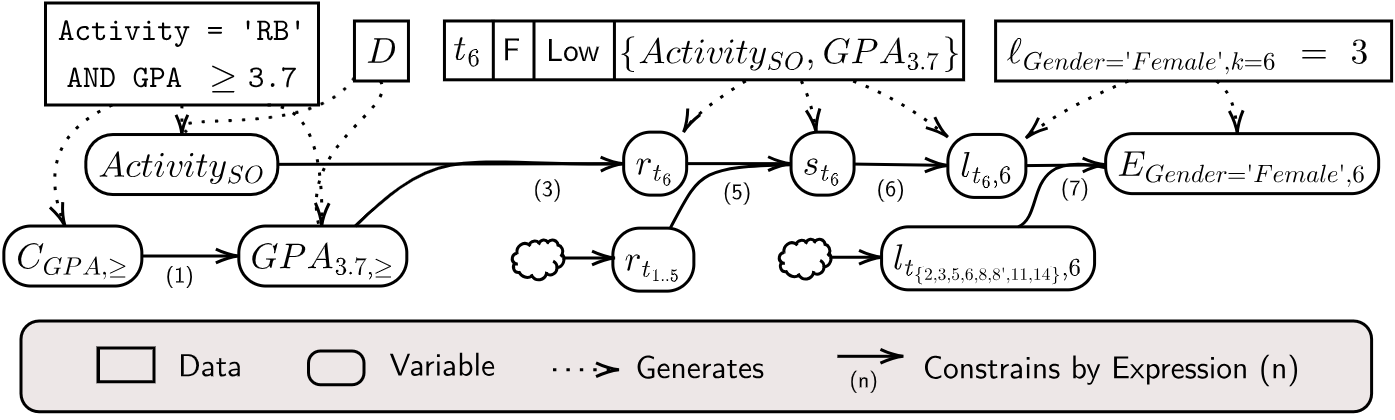
\includegraphics[width=0.75\linewidth]{figures/example_summary.png}
    \caption{Diagram illustrating the expression generation for our running example. The predicate {\tt Activity = `RB' AND GPA $\geq$ 3.7} generates the variables $Activity_{SO}$ and $GPA_{3.7, \geq}$ as `SO' and $3.7$ are values that appear for those attributes respectively in the database $D$. $C_{GPA, \geq}$ is also generated by the predicate to hold the new constant of the predicate, and constrains the value of $GPA_{3.7, \geq}$ by (\ref{eq:value_bounds_inline}). The tuple $t_6\in \widetilde{Q}$ generates the variable $r_6$, whose value is constrained through (\ref{eq:tuple_in_ranking_inline}) by the values of $Activity_{SO}$ and $GPA_{3.7, \geq}$ due to its lineage. It also generates the variable $s_6$, which is then constrained by the value of the $r_t$ values for the tuples that rank better than it, i.e., $r_{t_{1..5}}$, through (\ref{eq:position_in_ranking_inline}). Finally, the constraint $\lb{Gender=`Female'}{k=6} = 3$ combines with $t_6$ to generate the variable $l_{t_{6},6}$ which is constrained by the value of $s_{t_6}$ by (\ref{eq:in_prefix_inline}). The constraint generates the variable $E_{Gender=`Female',6}$ which is constrained through (\ref{eq:tuples_to_satisfy_inline}) by the values of all the $l_{t, 6}$ variables for which $t$ is a part of the group (listed in \Cref{ex:deviation}).}
    \label{fig:example_summary}
    \vspace{-0.5cm}
\end{figure}


    


\paragraph*{\textbf{Model limitation}}
\label{sec:query_class_lims}
Given an input to our program, we construct a MILP program. The correctness of the solution generated by the program, as stated in \Cref{thm:bounded-deviation}, relies on three properties. First, every possible refinement may be represented as an assignment to the variables of the program. Second, the tuples in the output of any potential refinement are in the same relative order, and finally, every tuple in the output satisfies all the predicates of the corresponding refinement. We define the problem for SPJ queries, and thus, our model is designed to handle SPJ queries, and these properties hold for them. We note that supporting other classes of queries may require modifications to the problem definition as well as to our proposed model. For instance, in union queries, it is enough for a tuple in the output to satisfy the predicates of one branch of the union, in contrast to the third property. This may be handled straightforwardly, as noted in \Cref{sec:background}. Handling nested queries is more challenging since they may contain multiple selection statements at different nesting levels. The problem definition should first be extended to properly define how such a query can be refined, e.g., whether refinements at different nesting levels are allowed. Our proposed model cannot capture the refinement of selection statements in different nesting levels and, therefore, does not fulfill the first property. Moreover, if the {\tt ORDER BY} clause relates to an inner query, refining the inner query may change the relative order of the tuples in contrast to the second property.










\section{Optimizations}
\label{sec:optimizations}
In Section~\ref{sec:search}, we have presented a MILP formulation designed to solve the \problem{} problem. While this approach enables us to leverage existing MILP solvers that can solve the problem efficiently, they often encounter difficulties when dealing with extensive programs (containing numerous expressions), and a large number of variables~\cite{QFix}. While the number of expressions and variables in the MILP we generate is linear in the data size, MILP solvers struggle to scale and solve the generated programs as we show in Section~\ref{sec:experiments}. %



To this end, we propose three optimizations for the construction of the MILP problem: one is a general optimization that applies in all cases, and the other two are limited to some cases. The first optimization is relevancy-based and removes from consideration tuples that are irrelevant to determining the satisfaction of the constraint set. The second optimization reduces the number of binary variables in the MILP problem by combining redundant variables. This optimization cannot be applied for queries with a {\tt DISTINCT} statement. %
The third optimization relaxes the expression used to determine the score of a tuple in the new ranking. This optimization is only applicable to tuples belonging to groups with only lower-bound or only upper-bound constraints, but not both.


\paragraph*{\textbf{Relevancy}}
We propose a relevancy-based optimization to reduce the number of expressions and variables in our problem.
Recall that we use $k^*$ to denote the maximal $k$ that appears in the constraint set $\constraints$. Then, by removing tuples that could never appear in the top-$k^*$ in any refinement, we are able to avoid adding their variables and expressions to our problem. We determine the relevancy of these tuples by selecting the top-$k^*$ of the groups of tuples that share the same lineage. Let $[\prov(t)]$ be the equivalence class of tuples that share the same lineage as a tuple $t$. Then for a tuple $t$, let $T(t)$ be the ranking generated by ranking the tuples of $[\prov(t)]$ according to the {\tt ORDER BY} clause of $Q$. We see trivially that it is not possible for tuples past position $k^*$ in $T(t)$ for all $t$ in $\widetilde{Q}(D)$ to be included in the top-$k^*$ of any refinement. Thus, it is sufficient to consider only the top-$k^*$ of $T(t)$, denoted by $T(t)_{k^*}$, in the generated program, and we replace $\widetilde{Q}(D)$ in the expressions referencing it in Figure~\ref{fig:milp} with $\bigcup_{t \in \widetilde{Q}(D)} T(t)_{k^*}$ ranked according to the {\tt ORDER BY} clause of $Q$. 



\begin{example}\label{ex:optimization1}
    Consider $t_{14}$ from Table~\ref{tab:joined}. Its equivalence class $[\prov(t_{14})]$ is the set $\{t_7, t_{10}, t_{14}\}$. Assume we are interested in satisfying a single constraint $\lb{Gender=`Female'}{k=2} = 1$. Note that the tuple $t_{14}$ can never appear in the top-$2$ of any refinement query, as any refinement that includes $t_{14}$ includes tuples with its same lineage, i.e., $t_7$ and $t_{10}$. Therefore, it is safe to remove all variables and expressions related to $t_{14}$ from consideration.
\end{example}
This optimization is most effective when $k^*$ is small, and there are few lineage equivalence classes. In \Cref{sec:experiments}, we show that this is often the case in queries over real data sets. We further demonstrate the effect of $k^*$ on the running time in \Cref{fig:time_vs_k}.



\paragraph*{\textbf{Selecting lineages}} 
Recall that the program we generate includes a binary variable $r_t$ for each tuple in $\widetilde{Q}(D)$. However, tuples sharing the same lineage all have equal values for their $r_t$ variables. Therefore, we can use a single variable for all tuples in the same lineage equivalence classes. 

\begin{example}
    To demonstrate this idea, consider the \running{} without its {\tt DISTINCT} statement and consider again the tuple $t_{14}$ with its equivalence class shown in Example~\ref{ex:optimization1}. If $t_{14}$ satisfies the selection condition of a refinement on the \running{}, then $t_7$ and $t_{10}$ must satisfy the conditions as well, as they share the same lineage. Therefore, we have the equivalence $r_{t_{14}} = r_{t_7} = r_{t_{10}}$. The variables $r_{t_7}$ and $r_{t_{10}}$ are then made redundant, as they always have the same value as $r_{t_{14}}$. 
\end{example}

In order to avoid such redundancy, instead of constructing the set of $r_t$ variables, we construct a set of variables $r_{[\prov(t)]}$ for every tuple $t$ in $\widetilde{Q}(D)$. Using (\ref{eq:tuple_in_ranking_inline}) as a basis, we are able to model $r_{[\prov(t)]}$ being assigned $1$ if and only if the tuples in $[\prov(t)]$ satisfy the selection condition of the corresponding refinement query.
 Instead of constructing expression (\ref{eq:tuple_in_ranking_inline}) for each tuple in $\widetilde{Q}(D)$, we construct the following expression for each $r_{[\prov(t)]}$ variable:
    $0 \leq \sum_{p \in \prov(t)} p - |\conds(Q)| \cdot r_{[\prov(t)]} \leq |\conds(Q)| - 1$.
Furthermore, in order to ensure that the $s_t$ values are modeled as before, we modify (\ref{eq:position_in_ranking_inline}) by changing $r_t$ to $r_{[\prov(t)]}$ and $r_{t'}$ to $r_{[\prov(t')]}$.
We note that this optimization cannot be applied if the input query includes a {\tt DISTINCT} statement,
as we need this information in order to not select tuples that already have at least one tuple sharing its distinct value(s) in the output.

\paragraph*{\textbf{Relaxation for single-constraint-type tuples}}
We present another optimization that is possible when a tuple belongs to groups that have only either lower-bound ($\ell$) or upper-bound ($\mathscr{u}$) cardinality constraints made on them. We define the set of tuples belonging only to groups with lower-bound constraints as 
$L = \{ t \in \widetilde{Q}(D) \mid \not\exists (\ub{G}{k} = n) \in \constraints, t \in \widetilde{Q}(D) \cap G \}$.
We define a similar set $U$ for upper-bound tuples, replacing $\ub{G}{k} = n$ in the quantifier with $\lb{G}{k} = n$. Then, for a tuple $t \in L$, we relax expression (\ref{eq:position_in_ranking_inline}) to 
$1 + |\widetilde{Q}(D)| \cdot (1 - r_t) + \sum_{t' \in \widetilde{Q}(D), \widetilde{Q}(D)(t') < \widetilde{Q}(D)(t)} r_{t'} \leq s_{t}$. For tuples in $U$ we set an upper bound instead ($\geq s_t$). This relaxation makes finding feasible solutions for this model easier and may be used by presolving techniques in MILP solvers.

In order to understand why this maintains the correctness of our solution, consider the lower-bound constraints. Intuitively, we can allow the $s_t$ variables of tuples belonging to the group defined in the constraint in a given top-$k$ to be assigned a value larger than the position of $t$ in the ranking, as this could only result in a higher deviation for lower-bound constraints as determined by (\ref{eq:max_deviation_inline}). Suppose the deviation as calculated by (\ref{eq:max_deviation_inline}) is higher than the true deviation of the corresponding refinement. Then, the refinement returned by the MILP is still a correct answer as (\ref{eq:max_deviation_inline}) bounds the calculated deviation by the input $\varepsilon$ value, and therefore the true deviation of the corresponding refinement cannot be more than $\varepsilon$. On the other hand, if $s_t$ were assigned a value {\it smaller} than the position of $t$ in the ranking of the corresponding refinement's output, then the deviation as calculated by (\ref{eq:max_deviation_inline}) may be lower than that of the true deviation of the corresponding refinement, which could cause the MILP to return a refinement with a deviation higher than permitted. 
The case for upper-bound constraints is symmetric.





